\chapter[Tchaikovsky and \textit{The Seasons}, Op. 37a]{Pyotr Ilyich Tchaikovsky - June: Barcarolle from \textit{The Seasons}, Op. 37a (1875)}

Pyotr Ilich Tchaikovsky (1840-1893) was a leading Russian composer during the nineteenth century. Born in Votkinsk, Russia, Tchaikovsky moved with his family several times, including to Moscow and St. Petersburg, as his father searched for a job\autocite{Burkholder_Grout_Palisca_2014}. This did not dissuade Tchaikovsky from attempting to pursue a serious musical study, as he studied at the St. Petersburg Conservatory between 1862-1865, and then left to Moscow, where he received a teaching position at Moscow's Conservatory. During his time at the Moscow Conservatory, he composed his work \textit{The Seasons}, twelve character pieces for piano. A character piece is a type of program music. Program music is defined as a type of music which tells a story, able to illustrate various literary ideas or evoke pictorial scenes\autocite{Kennedy_Kennedy_Rutherford-Johnson_2013_programme_music}, and this definition can be expanded to include all music which attempts to represent some type of extra-musical material or concepts without spoken words\autocite{Scruton_2001}. The term ``program music'' was introduced by Franz Liszt, also the creator of the term \say{symphonic poem}, to describe the most characteristic aspect of program music. He described program music as music which the composer can both guard the listener against the ``wrong'' interpretation of the music, and also direct the listener's attention to the ``proper'' ideas of the piece as a whole or a particular piece of it. Contrasted with absolute music, music without these extra-musical concepts, program music is best characterized by its attempt to depict objects and events, not merely echoing or imitating these. In some cases, these pieces may attempt to literally evoke the scene of some type, with Tchaikovsky does to excellent effect with his June Barcarolle from \textit{The Seasons}. A character piece is designed to convey a specific allusion, atmosphere, mood, or scene, without text, stage action, or other program assistance\autocite{Temperley_2011}. The Romantic era (during the nineteenth century) encouraged literary influences in music, and nationalism of the time led composers, including Tchaikovsky, to evoke the folk music of various nations and ethnic groups. Tchaikovsky did this in his music by combining his Russian heritage with influences from Italian opera, French ballet, and Germany symphony and song, music similar to program music \autocite{Burkholder_Grout_Palisca_2014}.

Each piece in \textit{The Seasons} is of a different month of the year in Russia. The month of June is written in the style of a barcarolle. This is a song written in $\frac{6}{8}$ or $\frac{12}{8}$ time, typically sung by Venetian gondoliers, and has an accompaniment which suggests the rocking of a Venice gondolier\autocite{Latham_2011_barcarolle}. Within the June barcarolle, there is a slight deviation from the typical barcarolle piece. The piece is written in G Minor, and has an ABA form. Within the A section in Figure \ref{fig:t-first-three-lines}, we notice that this piece is actually in $\frac{4}{4}$ instead of the usual $\frac{6}{8}$ or $\frac{12}{8}$ time. This opening is marked as \textit{Andante cantabile}, or ``slowly sing'', to ensure the performer understands the sensitivity that must be brought to perform this piece. The time signature of $\frac{4}{4}$ and tempo marking \textit{Andante cantabile} gives a sense of pace, as well as the necessary combination of correct rhythm--as the Venetian gondolier ``sings''--and the treatment of the right hand's melody line. In the first two lines of the barcarolle, a dactylic (defined as a metrical pattern referring to a rhythm in which one strong syllable or beat is followed by two unstressed, or not strong, or short syllables or beats)\autocite{dactylic} pattern emerges, as clearly seen by Figure \ref{fig:t-first-three-lines}\autocite{Henle_2002}. Here, there is a clear long phrase which starts the dactylic pattern in bar two. The second beat of four through to the first three beats of bar six finish the first set of the dactylic pattern. This pattern repeats, in the last beat of bar six through to the first three beats of bar twelve. This twelve-bar phrase could form some type of period, ending of the first phrase group in the middle of bar six differs slightly from the ending of the second phrase group in the middle of bar twelve. Thus, there is an atypical form of the traditional period in the first twelve bars of the piece, found bracketed in red in Figure \ref{fig:t-first-three-lines}\autocite{Henle_2002}. 

Additional stylistic choices to create necessary sensitive and delicate sound, akin to physically being on a Venetian gondola and hearing the water and boat move, involve what is notated in Figure \ref{fig:t-a-section-style-choices}\autocite{Henle_2002}. First, there are several instances of a change in dynamics, with several crescendos and decrescendos marked, along with a \textit{piano} and \textit{forte} to obtain the right level of volume and balance from a performer. Specific to these measures is also the dynamic marker \textit{poco piú} (a marking meaning ``little more''), signifying a crescendo before a crescendo. The phrase peaks in bar fourteen on note F, and decrescendos down as the right hand approaches the note D. Other increases and decreases to volume follow through to the remainder of the A section, with the \textit{diminuendo} (a smooth decrease in volume) marker being the only other dynamic marker of note in the section.

\begin{figure}
  \centering
  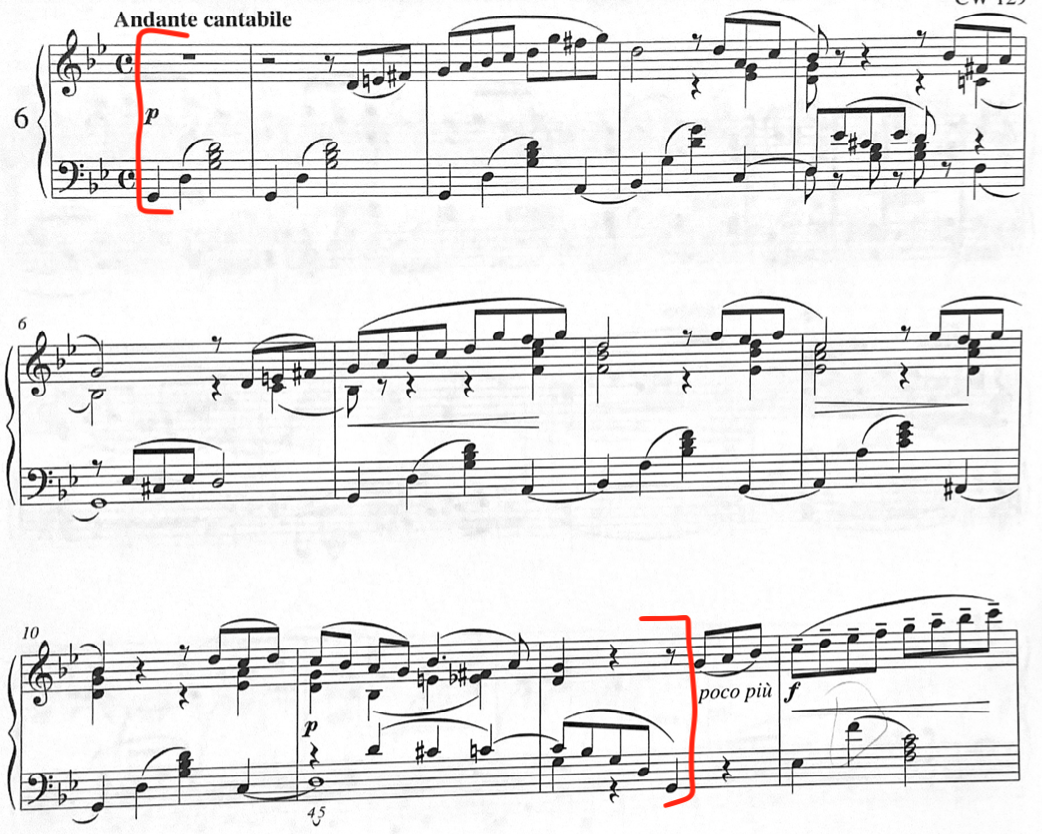
\includegraphics[width=0.5\textwidth]{t-first-three-lines.jpg}
  \caption{The first three lines, in Tchaikovsky's June: Barcarolle}
  \label{fig:t-first-three-lines}
\end{figure}

\begin{figure}
  \centering
  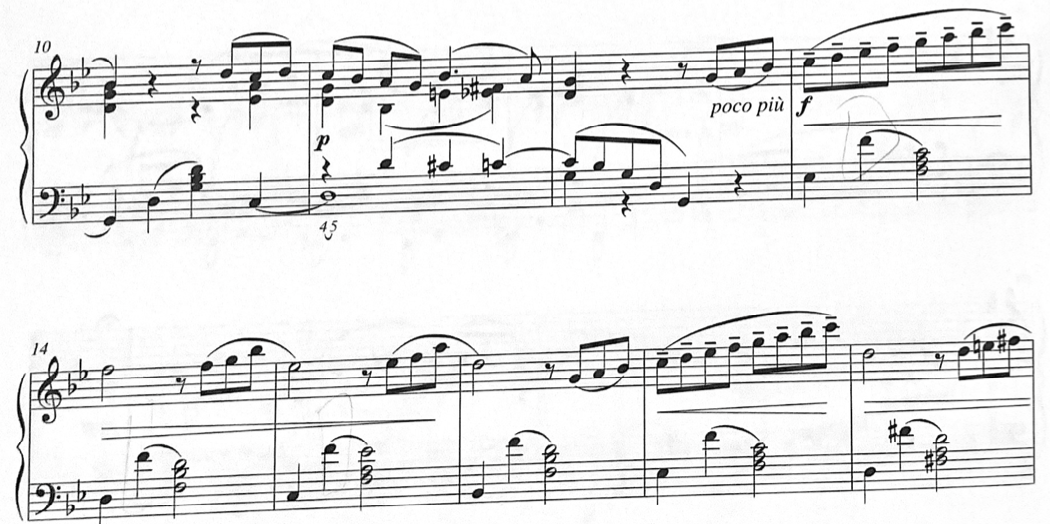
\includegraphics[width=0.5\textwidth]{t-a-section-style-one.jpg}
  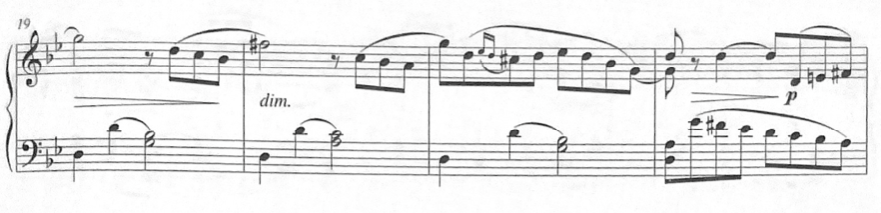
\includegraphics[width=0.5\textwidth]{t-a-section-style-two.jpg}
  \caption[Ornamentation Examples, in Tchaikovsky's June: Barcarolle]{Stylistic choices, written in to Tchaikovsky's June: Barcarolle}
  \label{fig:t-a-section-style-choices}
\end{figure}

\begin{figure}
  \centering
  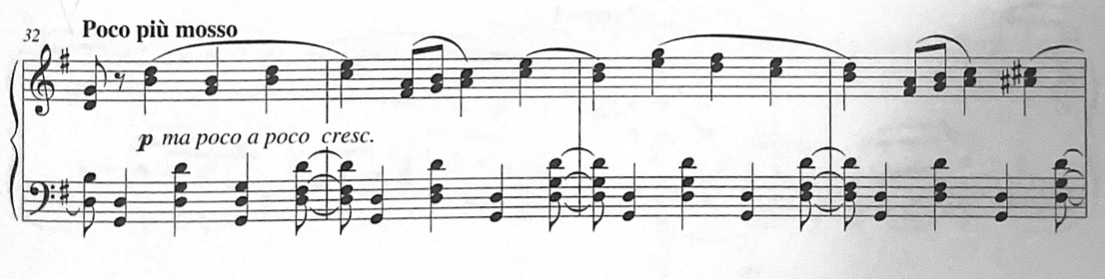
\includegraphics[width=\textwidth]{t-b-section-bars-32-35.jpg}
  \caption{Bars 32-35 of Tchaikovsky's June: Barcarolle}
  \label{fig:t-b-section-bars-32-35}
\end{figure}

\begin{figure}
  \centering
  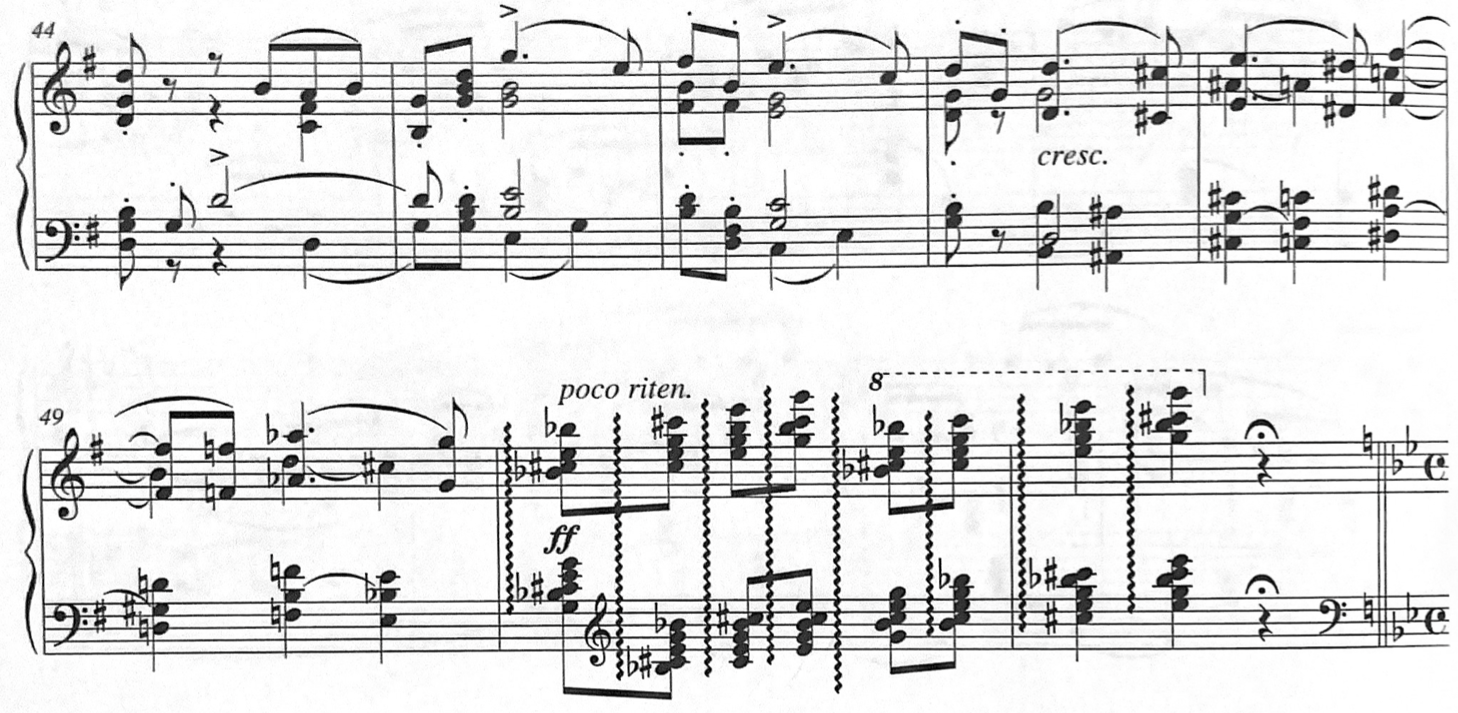
\includegraphics[width=0.7\textwidth]{t-b-section-bars-44-51.jpg}
  \caption{Bars 44-51 of Tchaikovsky's June: Barcarolle}
  \label{fig:t-b-section-bars-44-51}
\end{figure}


In the B section, the Venetian song continues, further immersing the listener into the song. The start of the section, as in Figure \ref{fig:t-b-section-bars-32-35}\autocite{Henle_2002}, begins with the tempo marking \textit{poco piú mosso} (roughly translating to ``a little bit faster''). It begins \textit{piano}, and as notated by the \textit{ma poco a poco crescendo}, the dynamic of the piece gradually increases slowly, until it reaches a peak at bar forty. The performer plays at \textit{forte}, indicating an increase in intensity within the Venetian gondolier's song, and a possible rockier nature to the gondola itself. This intensity is maintained through much of the section. Between bars 44-51, as in Figure \ref{fig:t-b-section-bars-44-51}\autocite{Henle_2002}, there are several other rhythmic and harmonic notations which the performer must keep in mind as well to maintain the necessary level of intensity and dramatization of the gondolier's song. Differently accented notes along with slurring certain lines contribute to the overall feeling of unsteadiness while the gondola floats its way down the Venice canal. Bars 44-46 are examples, as there are notes in both hands which begin as accented notes, and are followed immediately by slurred notes in short two-note phrases. Along with the staccato notes spread out in this figure, as well as the crescendo found in bar 47, the paddles of the gondola are heard in the background. The gondolier's singing is prominent above the sounds of the water in the canal and the rowing of the gondola itself, as the gondolier's singing becomes more dramatic and louder, through bar forty-seven's crescendo, and through to the arpeggiated chords in bars 50-51. The B section ends, with the arpeggiated chords of Figure \ref{fig:t-b-section-bars-44-51}\autocite{Henle_2002} becoming gradually slower with the \textit{poco ritenuto} tempo marking, culminating in a dramatic quarter-note length final note, and an extended quarter-note length rest (this extension is known as a fermata).

\begin{figure}
  \centering
  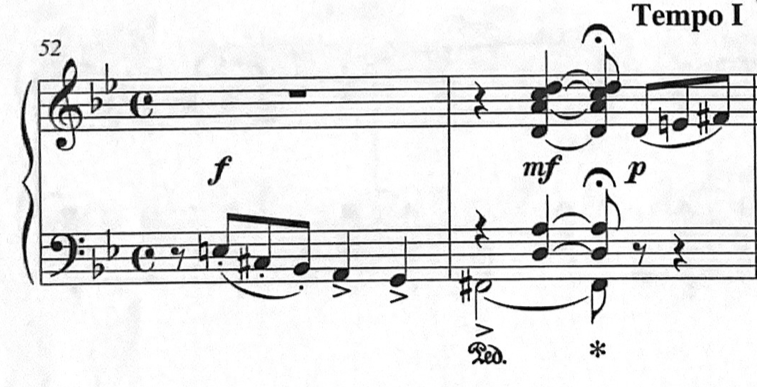
\includegraphics[width=0.5\textwidth]{t-transition-section.jpg}
  \caption[Transitioning between B section and A' section in Tchaikovsky's June: Barcarolle]{The transition section of Tchaikovsky's June: Barcarolle}
  \label{fig:t-transition-section}
\end{figure}

Slightly before the return of the A section, there is a brief measure and a half transition section. As in Figure \ref{fig:t-transition-section}\autocite{Henle_2002}, there is a descent is the harmonic line in the left hand, with bar 52 to be played in \textit{forte}, and the second beat of bar 53 played in \textit{mezzo forte}. This transition section reduces the intensity and high-energy that was found in the B section, moving it back to the gentle sensitivity of the A section. This is helped by the three note slur which starts this section, and the fermata over the two tied quarter notes which ends the section. Programmatically, the highest peak of the Venetian gondolier's song is over. The block chords of the B section give way for the broken chords style in the A section, with block chords in the transition section only signifying the transition to the A section. The gondola is able to continue on its journey, gentling floating down the Venice canals with the help of the gondolier.

\begin{figure}
  \centering
  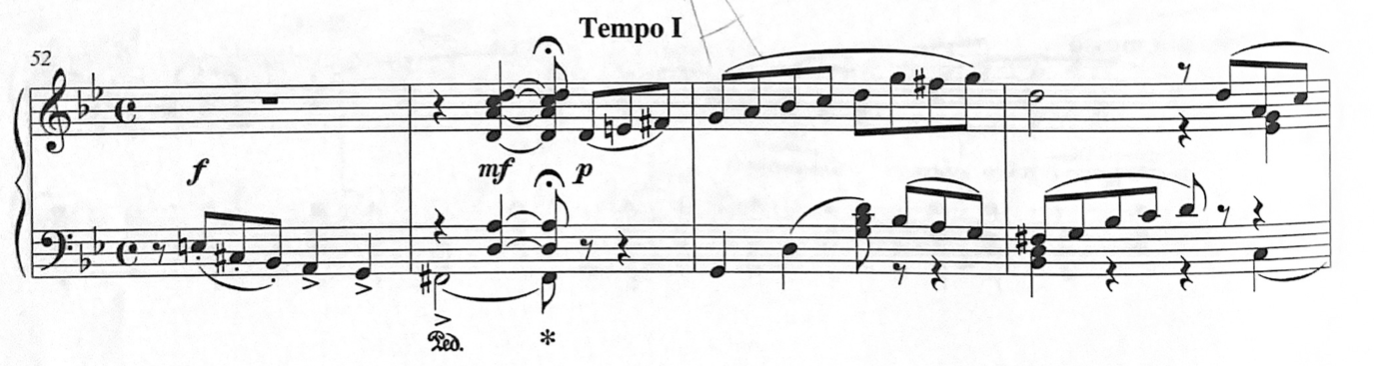
\includegraphics[width=0.5\textwidth]{t-a-prime-beginning.jpg}
  \caption{A' Section in Tchaikovsky's June: Barcarolle}
  \label{fig:t-a-prime-beginning}
\end{figure}


Finally, the A' begins, featuring a return of many of the material that was treated in the first A section. The tempo of the piece goes back to \textit{Tempo I}, the A section's tempo and the original tempo of the piece. The dactylic nature of the A section also returns in A', and as in Figure \ref{fig:t-a-prime-beginning}\autocite{Henle_2002}, the Venetian gondolier's song has lessened in intensity and energy, with the listener only vaguely aware of the left hand's slurred motion which simulated the rocking of the gondola, and the gondolier slowly bringing the song to an end. Towards the end of the A' section, there is a return of the block chords which featured heavily in the B section, as in Figure \ref{fig:t-a-prime-ending}\autocite{Henle_2002}, starting with the marks which bracket the beginning of the ending in red. The Venetian gondolier's song, which is played in the right hand, decreases in volume to \textit{pianissimo} through a decrescendo, and turns to be a melody which is low in pitch and much more mysterious than it had been previously. The motion of the gondola also changes slightly, as the left hand's notes are no longer dactylic, beginning in measure 92. The left hand notes begin to be played in pairs, rather than groups of three, symbolizing the literal end of the gondola right which the listener is on. The block chords which end the piece in the right hand, from measures 92 to the end in Figure \ref{fig:t-a-prime-ending}\autocite{Henle_2002}, also signify that the gondolier's song is ending, and the listener is ready to disembark the gondola.

\begin{figure}
  \centering
  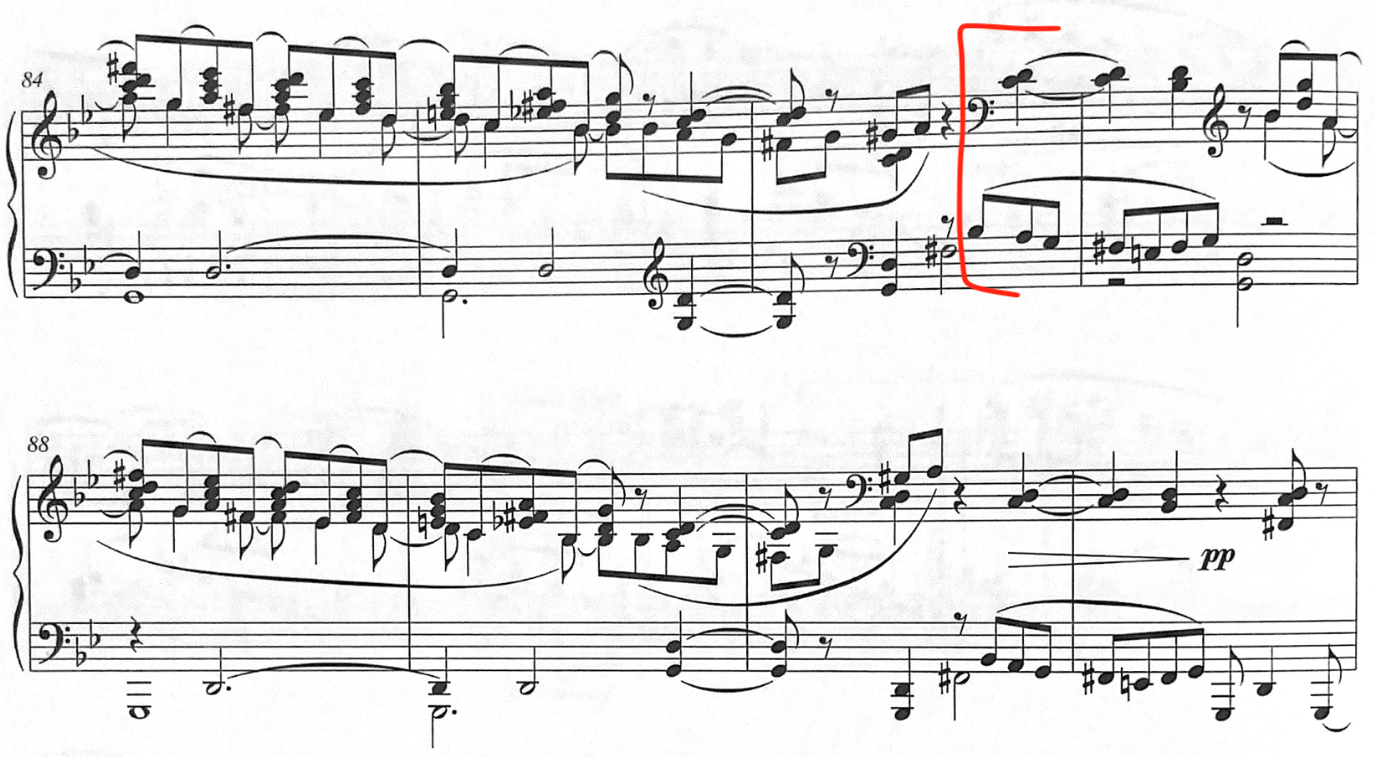
\includegraphics[width=0.8\textwidth]{t-a-prime-end-1.jpg}
  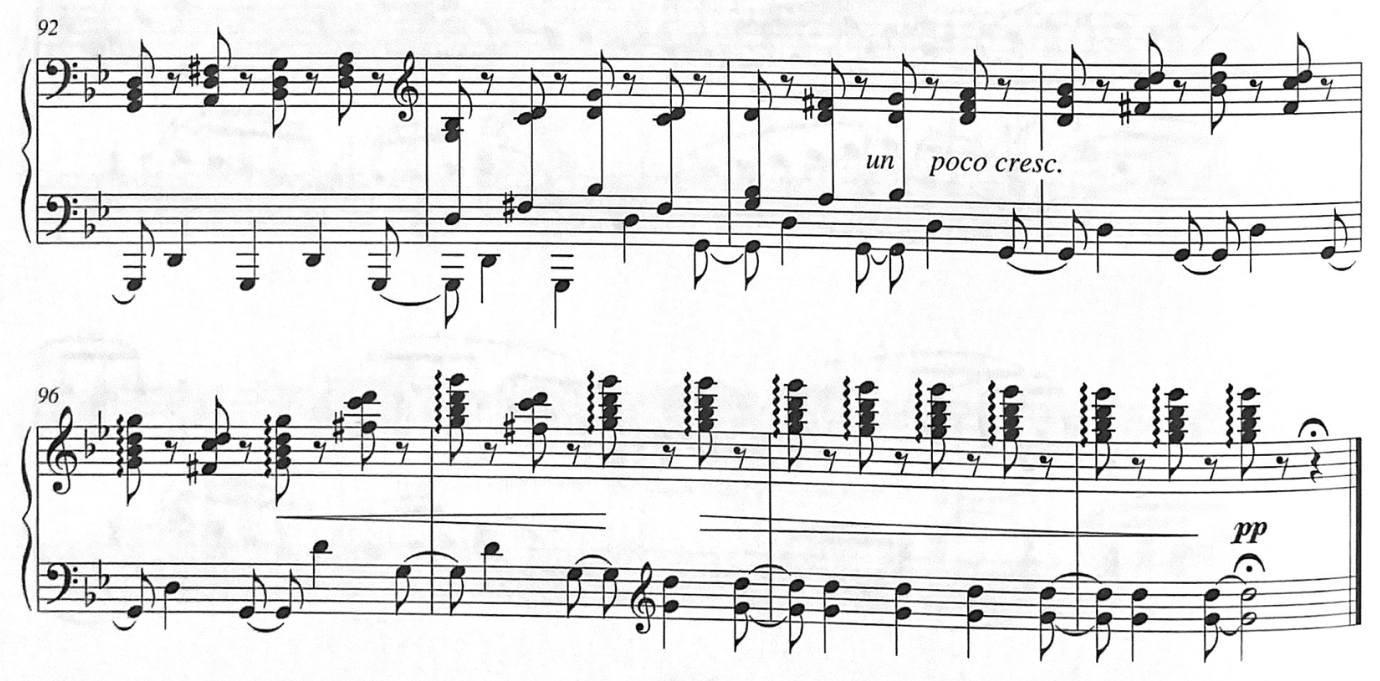
\includegraphics[width=0.8\textwidth]{t-a-prime-end-2.jpg}
  \caption{The ending of Tchaikovsky's June: Barcarolle}
  \label{fig:t-a-prime-ending}
\end{figure}

\section{A Gondolier's Song}

The June: Barcarolle is a character piece, meant to emulate the experience of being on a gondola ride through the canals of Venice, while a gondolier sings a folk-song. Within the first five bars of the piece, of Figure \ref{fig:t-first-three-lines}\autocite{Henle_2002}, the left hand's motion is similar to that of a rocking boat. Measures one and two feature a rhythmic pattern of two quarter notes and a half note, with the second quarter note slurred into the half note. Then, measures three and four change and become a rhythm of four quarter notes, with the last quarter note of the measure slurred into the first quarter note of the next measure. On the fourth beat of measure four, the last quarter note of the left hand is slurred into the first eighth note of measure five, which begins the rockier motion of the canal's water.

It is through this emulation of the gondolier's strokes that the listener is transported themselves to the gondola ride hosted by the gondolier. As the right hand melody enters on beat three of measure two, and the Venetian gondolier begins to sing, there is a notable slow and unnerving quality to the gondolier's song. The gondolier introduces a gloomy, almost spooky atmosphere to the piece, which I aim to replicate during the A and A' sections. Though the tonic key of the piece is G Minor, as seen by G and D being the beginning two notes, Tchaikovsky employs the use of the raised seventh scale degree F\musSharp{}. Through the A and A' sections, I use this raised scale degree seven to emphasize the nature of the gondolier singing, without placing emphasis on the note itself. The note F\musSharp{} appears frequently through the two sections. Along with it, I also use a large range of dynamic contrast when additional melodic material is introduced on beat four of measure 12. The dynamic contrast changes from being \textit{piano} (with some crescendos and decrescendos) to being marked \textit{forte}, as in Figure \ref{fig:t-a-section-style-choices}\autocite{Henle_2002}. It is from here in measure 12 that I begin playing with a clear contrast in dynamics, and introduce a slight difference in tone as well. Prior to measure 12, my playing involves a warm feeling, relying on the notes around Middle C and below to bring about a feeling of uncertainty and spookiness. However, once I get to beat four of measure 12, and notes above a $C_4$ become more common, I lose the warm tone in favor of a sound that is brighter, and more closely follow the dynamic markings. In Figure \ref{fig:t-a-section-style-choices}\autocite{Henle_2002} as the note G begins the melody line, and the line rises, there is a marked \textit{forte}, along with several long crescendos and decrescendos. As I play with a bright, but also still slightly warm sound, the gondolier's song begins to sound akin to a tangent within a story. The first eleven measures of the piece are consistent in character, with a warm sound, played \textit{piano}, as the gondolier floats the listener down the canals of Venice. Then, in measures 12-22, the sound changes. It sounds as if the gondolier becomes lost in the story that they are telling, and has a sudden remembrance of a lost memory, which brought them happiness in the past, thus having a brighter tone in the song. This temporary happiness at a forgotten memory becomes dull once again in measure twenty-two, as if the gondolier remembers themself, and returns to the dramatic, and gloomy atmosphere of the song they intended to sing.

The B section of this piece begins in measure thirty-two, as in Figure \ref{fig:t-b-section-bars-32-35}\autocite{Henle_2002}. The character of this section is like that of the bright sound seen in the middle of the A section, except this section serves a different purpose. Rather than a lost memory, the B section is the climax of the story of the song the gondolier sings. There is more action, as both hands are now playing a mixture of moving quarter notes and eighth notes, rather than only the melodic line containing moving eighth notes (Figure \ref{fig:t-b-section-bars-32-35}\autocite{Henle_2002}. I also portray this faster motion, with the \textit{piano ma poco a poco crescendo} (``piano, but little by little crescendo'') and groups of four quarter notes in the melody line that are grouped together. Both of these ornamental aspects (the group of four quarter notes, and the dynamic marking to slowly increasing the dynamic volume of the section) are necessary, as I emulate the excitement of the gondolier's song. Towards the end of the B section, the gondolier sings with more syncopation to their rhythm (as in Figure \ref{fig:t-b-section-bars-44-51}\autocite{Henle_2002}). Like in the second beat of measure forty-five, a rhythmic pattern of dotted quarter notes slurred into an eighth note emerges. This emulates the absolute climax of the song's story. After the phrase which includes several sets of dotted quarter notes slurred into eighth notes, this is the ending of the B section. This ending involves two measures of rolled eighth notes, emphasizing the height of the song's drama the gondolier sings about. With the prolonged quarter rest which ends the B section, I play the short, one-measure long transition to the A' section as contemplative, as the protagonist of the gondolier's story returns back to thematic material of the A section, but this time as the resolution of the story.

This one-bar transition section is notable as a stark contrast to how the B section ended. While I played the rolled eighth notes of the B section quickly getting increasingly louder, while also slowing slightly with the \textit{poco ritardando}, culminating into a rolled quarter note. The transition section is a slurred three-note long eighth note, two accented quarter notes, and a held half note in the left hand. The right hand rests, but then in measure 53 (in Figure \ref{fig:t-transition-section}\autocite{Henle_2002}), enters very dramatically, with a tied quarter note into an eighth note. This is the entrance that I increase the dramatic nature of, as it is an entrance played \textit{mezzo forte}, and the next phrase needs to be played \textit{piano}.

Then, as the A' section ends, in beat four of measure 86, there is another change in thematic material. In bars 92 through to the end of the piece, as in Figure \ref{fig:t-a-prime-ending}\autocite{Henle_2002}, the left hand's harmony becomes more dichotomous in nature. Quarter notes and eighth notes begin to alternate, in a slightly syncopated pattern. As this is no longer emulating the rocking motion of the gondola as the melody was in the A section, and the beginning of the A' section, the listener is approaching the end of the gondola ride. The motions become rockier as the listener disembarks from the gondola, and the gondolier finishes singing their song, with the melody rising in pitch to match a dramatic ending. I play this section to indicate the ending of the boat ride, to imply unsteadiness. The harmony line is no longer smooth nor reliable, instead turning to be syncopated in rhythm, and the melody line matches this. This unsteadiness is due both to the listener's physical leave of the gondola, as well as the protagonist in the gondolier's story becoming crazed. Drawn out dynamic changes, and the melody and harmony line alternating in sounding both contribute to this feeling, which I emphasize. I follow the steady increase in dynamic volume, creating a full sound in the last three measures of the piece, as the rolled quarter notes in the right hand and un-rolled quarter notes in the left hand take turns in sounding. I end the piece with a dramatic ending, suitable for the gondolier ending their song, with the right hand's melody sounding quiet yet full, and the left hand's harmony extending a tied eighth note and half note. There is a sense of unfinished business, as seen by the extended quarter note which technically ends the piece. 
